% This is a sample document using the University of Minnesota, Morris, Computer Science
% Senior Seminar modification of the ACM sig-alternate style. Much of this content is taken
% directly from the ACM sample document illustrating the use of the sig-alternate class. Certain
% parts that we never use have been removed to simplify the example, and a few additional
% components have been added.

% See https://github.com/UMM-CSci/Senior_seminar_templates for more info and to make
% suggestions and corrections.

\documentclass{sig-alternate}
\usepackage{color}
\usepackage{graphicx}
\usepackage{mathtools}
%\usepackage[colorinlistoftodos]{todonotes}

%%%%% Uncomment the following line and comment out the previous one
%%%%% to remove all comments
%%%%%\newcommand{\comment}[1]{}
\newcommand{\comment}[1]{{\bf \tt  {#1}}}
%%%%% NOTE: comments still occupy a line even if invisible;
%%%%% Don't write them as a separate paragraph
\newcommand{\todo}[1]{\textcolor{magenta}{\comment{Todo: {#1}}}}

\begin{document}

% --- Author Metadata here ---
%%% REMEMBER TO CHANGE THE SEMESTER AND YEAR
\conferenceinfo{UMM CSci Senior Seminar Conference, May 2015}{Morris, MN}

\title{Monte Carlo Tree Search and Its Applications}

\numberofauthors{1}

\author{
% The command \alignauthor (no curly braces needed) should
% precede each author name, affiliation/snail-mail address and
% e-mail address. Additionally, tag each line of
% affiliation/address with \affaddr, and tag the
% e-mail address with \email.
\alignauthor
Max Magnuson\\
	\affaddr{Division of Science and Mathematics}\\
	\affaddr{University of Minnesota, Morris}\\
	\affaddr{Morris, Minnesota, USA 56267}\\
	\email{magnu401@morris.umn.edu}
}

\maketitle
\begin{abstract}

\end{abstract}

\keywords{Monte Carlo Tree Search, Heuristics, Upper Confidence Bounds, Artificial Intelligence}

\section{Introduction} 
In 1997 the field of artificial intelligence(AI) experienced a monumental breakthrough when IBM's Deep Blue defeated Garry Kasparov, a reigning grand master, in a chess match\cite{TheGrandChallenge}. They were able to achieve this by using brute force deterministic tree searching methods combined with human knowledge. The human knowledge allows for the computer to evaluate moves properly, and then populate a tree to search for the best move. This event really demonstrated to the world the power of computers and artificial intelligence. 

While computers are capable of outplaying the top players of chess, they struggle when it comes to board games like Go\cite{TheGrandChallenge}. Go is a board game that originated in China, and it has a strong professional community. It is a game about positional board advantage which is something traditional AI approaches struggle with evaluating. This is because moves in Go tend to have very long dependencies. A single move may have major effects on moves 50 to 100 moves down the line. Also Go has significantly more moves available to the player at anyone time than chess. These problems cause deterministic approaches to perform poorly. It is just too much for those approaches to efficiently handle.

People have started turning to alternative methods to approach Go. One such method, Monte Carlo tree search(MCTS) has had a lot of success in Go. MCTS eschews the typical brute force tree searching methods, and it utilizes statistical processes and heuristic approaches to decide what move to make. In 2009, for the first time ever, a computer defeated a top professional Go player in a 9x9 game\cite{TheGrandChallenge}. It took twelve years since Deep Blue defeated Garry Kasparov for AI to achieve its first major victory in Go, and it was only on the smallest board that Go is played on.

MCTS has been growing in popularity in recent years, and it demonstrates a lot of promise. In this paper we will be examining MCTS and a few of its applications.  
\section{Background}
MCTS combines the random sampling of traditional Monte Carlo methods with tree searching. The random sampling is used to construct a game tree. This tree will be traversed based on statistical processes, and the MCTS method relies on the convergence of the tree to reliably choose the best move. MCTS is a heuristic method and as such it will not always find the most optimal move, but it has a reasonably high success of choosing moves that will lead to greater chances of winning.
\subsection{The Tree Structure}
MCTS structures the game state and its potential moves in a tree. Each node in the tree represents the state of the game with the root node representing the current state. Each line represents a legal move that can be made from one game state to another. In other words, it represents the transformation from the parent node to the child node. Any node may have as many children as there are legal moves. For example, at the start of a game of Tic-Tac-Toe the root node may have up to nine children. One for each possible move. Each following child can only have one less child than its parent since the previous moves are no longer available as options.
\begin{figure}[h]
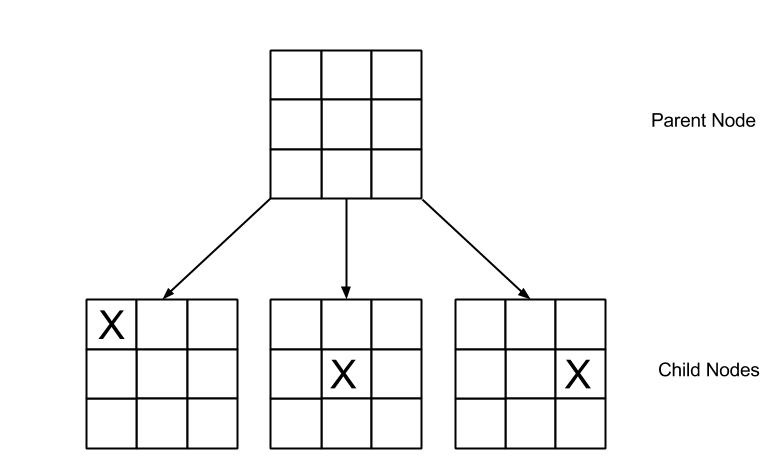
\includegraphics[height=5cm]{TicTacToeTree.jpg}
\centering
\caption{A small portion of what a tree represents}
\label{fig:TicTacToe}
\end{figure}

Figure \ref{fig:TicTacToe} represents the top portion of a tree for the game Tic-Tac-Toe. The AI is making the first move, so the source node is the first game board. Each child node represents the potential moves that can be made from the current game state. It is important to note here that those are only three of the potential nine child nodes.\todo{This somewhat contradicts what I say later on in the paper about UCT} MCTS does not have to look at every potential child node, nor will it want to for sake of efficiency. Once MCTS has decided which move to make, the source node of the tree will then become the child it chose. For example, if MCTS chose the left child in figure \ref{fig:TicTacToe}, then the new MCTS tree would start at that child and everything else that was branching off of the original parent node is discarded.

Along with the game state, each node encodes for a value that represents how favorable choosing a particular node is. This value comes from the respective values of the nodes that branch off of it. In the example of Tic-Tac-Toe we could assign any node that ends in a loss, a negative one, ends in a win, a one, and ends in a draw, a zero. When any of these values are discovered, then the rest of the tree that branches into that node can be updated with its value. So in this case, choosing the node with the greatest value, leads to a path with the greatest ratio of wins to losses. By doing this, it gives the AI the greatest chance of choosing a winning outcome.

\subsection{The Four Steps of MCTS}
The process of Monte Carlo tree search is split up into four processes: Selection, Expansion, Simulation, and Backpropagation. These four processes are iteratively applied until a decision from the AI must be made.

\todo{This section still needs a lot of work}

\textbf{Selection} - In the selection process, the MCTS algorithm traverses the current tree using a tree policy. A tree policy uses an evaluation function that prioritize nodes with the highest estimated value. 

\textbf{Expansion} - In expansion a new node is added to the tree as a child of the leaf reached in the previous step. Then a simulation is played out to determine the value of the newly added node.

\textbf{Simulation} - In this step, a simulation is played out according to the simulation policy. The policy randomly selects moves until either an end state or a predefined threshold is reached. Then based on the result of the simulation, the value of the newly added node is established. For example, a simulation of a node for Go would reach the end of a game(the end state), and then determine a value based on whether the player won, drew, or lost.

\textbf{Backpropagation} - Once the value of the node is determined, then as the name of this process implies, the rest of the tree can be updated. The algorithm will traverse back to the root node only updating the values of the nodes that it passes through. Only those nodes are effected because each node's respective value is an estimation of values of the nodes after them. For example, a particular node of a tree that encodes for the game Go contains a value that estimates how likely a player is to win or lose given that line of play. In other words, a higher value means that there are more potential games in which that player will win if that move is chosen.

\subsection{Upper Confidence Bound Applied to Trees(UCT)}
\todo{Get across that each unexplored node is explored before moving on, but only at each node that is visited. If a node is not visited again, that node's children will not be explored.}
The UCT is what the MCTS algorithm uses as a tree policy to traverse the tree. The goal of the UCT is to balance the idea of exploration versus exploitation. The concept of exploration promotes exploring many unexplored areas. This approach may explore many different paths on its way to finding the best decision. While this approach is useful to ensure that MCTS is not overlooking any potential paths, it can become very inefficient very quickly with games with a large number of moves. This is balanced with exploitation. The exploitation approach will tend to stick to one path that has the greatest estimated value. UCT balances these two ideas by exploring every unexplored node that it visits, but then it only visits nodes that yield the greatest estimated value.

 \begin{equation}
 \label{UCTequation}
 UCT(node) = \frac{W(node)}{N(node)} + \sqrt[c]{\frac{ln(N(parentNode))}{N(node)}}
 \end{equation}

When traversing the tree, Equation \ref{UCTequation} is applied to each of a node's children to evaluate the estimated value of that node\cite{ActionSelection}. N() represents the total number of simulations made at that node and the nodes branching off of it. W() represents how many of those simulations ended in a winning state. C represents an exploration constant that is found experimentally. The first part of the UCT takes into consideration the known estimated value of the node by determining the ratio of simulations won to total simulations. The second part of the UCT takes into consideration the unexplored nodes of the parent node by taking the ratio of the parent node's total simulations to the node's simulations.

\section{Using MCTS to play Go}

\subsection{Variations in Their MCTS Algorithm}

\subsection{Their Results}

\section{Using MCTS for Narrative Generation}

\subsection{Variations in Their MCTS Algorithm}

\subsection{Their Results}

\section{Using MCTS to play Mario}

\subsection{Variations in Their MCTS Algorithm}

\subsection{Their Results}

\section{Conclusions}

\section{Acknowledgements}

\section{References}

\subsection{Citations}

% The following two commands are all you need in the
% initial runs of your .tex file to
% produce the bibliography for the citations in your paper.
\bibliographystyle{abbrv}
% sample_paper.bib is the name of the BibTex file containing the
% bibliography entries. Note that you *don't* include the .bib ending here.
\bibliography{MaxMagnusonSeniorSeminar}  
% You must have a proper ".bib" file
%  and remember to run:
% latex bibtex latex latex
% to resolve all references

\end{document}
